\documentclass[conference]{IEEEtran}
\IEEEoverridecommandlockouts
% The preceding line is only needed to identify funding in the first footnote. If that is unneeded, please comment it out.
\usepackage{cite}
\usepackage{amsmath,amssymb,amsfonts}
\usepackage{algorithmic}
\usepackage{graphicx}
\usepackage{textcomp}
\usepackage{xcolor}
\usepackage{float}
\def\BibTeX{{\rm B\kern-.05em{\sc i\kern-.025em b}\kern-.08em
    T\kern-.1667em\lower.7ex\hbox{E}\kern-.125emX}}
% !TeX spellcheck = en_US 

\begin{document}

\title{Detection of Intersecting Machining Features via SSD on generic STL-Files\\}

\author{\IEEEauthorblockN{1\textsuperscript{st} Jan Nalivaika}
	\IEEEauthorblockA{\textit{UNC Charlotte} \\
		\textit{Energy Production \& Infrastructure Center}\\
		Charlotte, North Carolina, USA \\
		nalivaika@outlook.de}
	\and
	\IEEEauthorblockN{2\textsuperscript{nd} Dr. Joshua Tarbutton}
	\IEEEauthorblockA{\textit{UNC Charlotte} \\
		\textit{Energy Production \& Infrastructure Center}\\
		Charlotte, North Carolina, USA  \\
		joshua@bravoteam.tech}
	\and
	\IEEEauthorblockN{3\textsuperscript{rd} Dr. Martin Koerdel}
	\IEEEauthorblockA{\textit{Siemens AG.} \\
		\textit{T-REE-MDM}\\
		Munich, Germany \\
		martin.koerdel@siemens.com}
	}

\maketitle

\begin{abstract}
Industrie 4.0 is laying a new path for optimized machining and production.
The means of manufacturing achieve higher productivity due to increased inter-connectivity, high use of data and flexible manufacturing processes \cite{Shi.2021, Zhang.2018}. One of the most important areas in this transition to new manufacturing methods is automated manufacturing \cite{Gapinski.2009}. Self-aware machines optimize the individual process-steps, provide self-corrections and plan ahead without necessary human input \cite{Zhang.2018}.

Especially tool-path-planning, in the area of subtractive manufacturing, can benefit from a new and innovative ways of generating optimal tool-paths. Current tool-path planning algorithms do knowledge the existing machining features as standalone elements, which can result in inefficient paths with a unnecessary percentage of air-cutting time and thus loss of production capacity and profit \cite{Zhang.2018}.

The current state of the art provides a possibility of recognizing and locating multiple intersecting features but only on predefined STL-files with specific dimensions \cite{Zhang.2018, Shi.2021, Shi.2020}. This process can not be implemented into real-life production scenarios, as STL-files are unique and do not follow strict geometric rules \cite{CHAN}. 

Motivated by this problem, this paper provides a concept of recognizing and localizing intersecting machining features on various STL-files independent of orientation and size. The results show a sophisticated capability of handling various STL-files with different sizes, slopes and orientations. The architecture of this method is designed as such, that the Neural Network that is used for detecting the features can be exchanged easily, as soon as better trained options are available.\newline
\end{abstract}
\begin{IEEEkeywords}
	Feature Recognition, Machining-Features, SSD, Automated Manufacturing, Machine Learning
\end{IEEEkeywords}
\section{Introduction}
Due to the ever shortening product life cycle and more unique customer demands, the current production and manufacturing facilities are forced to adapt in order to fulfill the requirements and now be squeezed out of the market \cite{safi.2017}. Most factories are designed to produce a finite set of individual products in large quantities and can do so with high degree of efficiency and precision. When a company is requested to produce a unique part a lot of time is wasted due to the required setup and necessary human labor, as the available machines are not optimized for unique tasks. \cite{Oliveira.} \newline
One of the most prevalent ares where a lot of improvement can be expected, is the automated set-up process on milling operations. This process starts with converting a file-format that describes the final geometry of a part into instructions that a CNC-machine can interpret. As of now the algorithms that are embedded in most CAD/CAM-software suites do now take the machining features (MF) into account when generating tool-paths. This is due to the fact that these algorithms are not aware of the desired end result as they do not have the capability to recognize these MF and using them to create suitable tool-paths with the optimal tool. \cite{SalehM}
\section{State of the Art}

-https://ieeexplore.ieee.org/document/9222288 https://github.com/PeizhiShi/SsdNet
-A novel learning-based feature recognition method using multiple sectional view representation
-Featurenet: Machining feature recognition based on 3D convolution neural network
-Automatic feature recognition using artificial neural networks to integrate design and manufacturing: Review of automatic feature recognition systems
-
-
-
\section{Problem Formulation and Aim}
Analyzing the state of the art, reveals a lack of capability when it come to working with real-life STL-files. It requires a method of working with STL-files of various sizes, that can be positioned in different orientations relative to the axis and may contain angled faces. The goal is to build on the current possibilities of feature detection and add the required pre- and post-processing steps to enable the desires behavior, that can bring this method closer to the implementation in real-life production scenarios.
\section{Concept}
To implement the ability of handling various STL-files with different orientations and geometric shapes, multiple pre-possessing and subsequent post-processing steps have to be performed. Figure \ref{fig:flow} outlines the necessary steps.
\begin{figure}
	\begin{center}
	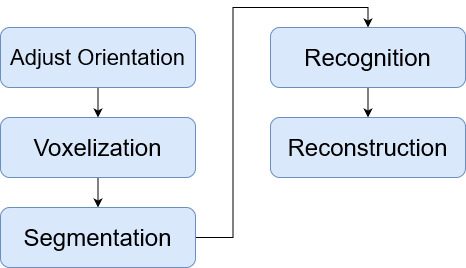
\includegraphics[width=0.7\linewidth]{pictures/flow.jpg}
	\caption{Conceptual workflow of pre-processing, recognition and post-processing }
	\label{fig:flow}
	\end{center}
\end{figure}

\subsection{Adjusting Orientation}
It is assumed that most STL-files are constructed in such a way where most area is facing one axis and most feature-symmetry-axis are parallel to one axis. For working with MF that are positioned on an angled surface, the following rotation has to be implemented. 

For optimal detection, the STL-file, has to be turned in such a way where the most surface area is facing one of the axis. This is required, as MF are mostly paced on flat surfaces and the detection of MF is only reliable when the viewing angle is orthogonal to the plane on which the feature is located. Viewing a MF at an angle, represents a distorted view and leads unreliable results. 

Finding the optimal angle to turn the STL-file around a specific axis is achieved by analyzing the normals of every facet. The area of facets that have an identical normal-vector are summed up and stored in a list. After that, the list that now only contains unique normals and the corresponding summed up area is sorted by the area. By going through the list and analyzing if a normal is parallel to the viewing angle, which is in that case an axis, it possible to identify whether the area is orthogonal to the viewing angle.

If a normal is not parallel to one of the axis and the "area to total-area"-ratio surpasses a certain threshold, the angle between two chosen coordinate-axis is calculated. The two obtained angles are used in a rotation matrix that is applied to all vertexes and normals of the STL-object. After that the file is stored under a new unique name. Optimally the name should give some information about the relation to the original STL-file. For example: "OriginalName\_39X\_49Y.stl", which indicates that that STL-file is turned by 39 degrees around the X-axis and 49 degrees around the Y-axis. The calculated angles are stored, as they can be used for placing bounding boxes on a 3D object for visualization of the detected MFs. This process can be repeated with the next normal that is not oriented parallel to a axis until all areas that are over a certain area-percentage were oriented orthogonal to one of the viewing angles.
\subsection{Voxelization}
The STL-file is transformed into a voxel model that is used in the subsequent step. At first the resolution of that voxel model has to be set. The resolution is defined by how many voxels are in one cubed millimeter. As every file can have a different ration of absolute dimensions to smallest-facet-dimension, its not possible to go by one standard resolution. To solve this problem, each facet of the STL-file is analyzed. From all facets the absolute minimal distance between two vertexes is determined. The following step is identifying the absolute length in the x-, y- and z-axis. The resolution is set by dividing the largest absolute dimension by the minimal distance between two vertexes. This value sets the number of voxels in the lagers dimension. 
By doing this calculation, it is made sure that the shortest distance is not lost in the voxel representation, during the voxelization-process. The calculated resolution can be multiplied by a scalar to increase the resolution if desired. It has to be considered that every increase in resolution will penalize the speed of the detection-process as more data will be created that has to be analyzed.    
Finally the STL-file is voxelized with the set resolution and stored. This process is repeated for every STL-file the was produced in the previous step.   
\subsection{Segemtation}
This process step is necessary as the NN can only use pictures with a set dimension for the detection process. 
To convert the now available voxel-files into adequate pictures from the corresponding viewing angles, the following steps have to be performed: At first the voxel-model is loaded and stored as a three-dimensional array. One side of the array is selected and an equally sized 2D-array is created. This 2D array will be saved as a picture. Each pixel, which is represented by a position in the 2D array, is set by counting how many voxel positions are empty until the first occupied voxel position in that direction. As an example: If the voxel model has a through-hole at a certain position, all empty voxel positions are counted. Every counted position is equivalent to lightening a pixel by a certain increment. That increment is defined by dividing 255 by the total depth of the voxel-model in that direction. 255 represents the maximum pixel-value of a picture with RGB-pixels. Initially all pixels are set to be completely black ([0,0,0]) and than lightened to create the perception of depth. Figure \ref{fig:HD_pic} gives a basic visual representation of this process.
\begin{figure}
	\begin{center}
		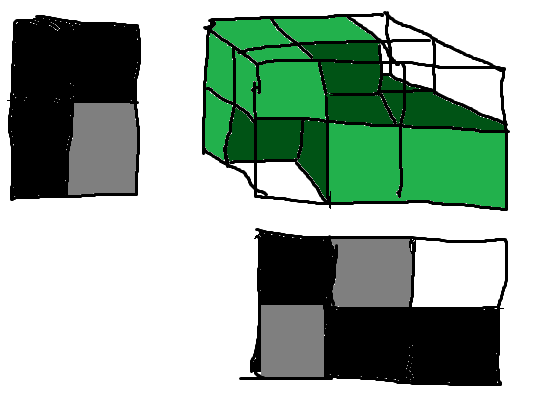
\includegraphics[width=0.7\linewidth]{pictures/HD_Picture_Process.png}
		\caption{Simplified representation of the creation of pictures from the voxel-models }
		\label{fig:HD_pic}
	\end{center}
\end{figure}
This process is repeated for the voxel-model of the STL-file that did not undergo any rotation, from every of the 6 directions (right, left, front, back, top, bottom).
The created pictures from the voxel-models, that are from now on referred as "main pictures", are saved under a unique name that is correlated to the viewing direction and the turned STL-file. For example: "OriginalName\_39X\_49Y\_Right.png" which indicated that this picture was made from looking at the voxel-model from the right (negative x-direction).
For all turned STL-files, it is not required to create all 6 pictures. Instead it is enough to only create a picture from the axis that the STL-file was turned to, as all other views are covered by other turned STL-file instances. 


The second step is subdividing the just created main pictures into smaller pictures that the NN can process. 
All main pictures are selected one by one and loaded into memory as a 2D array. Now, square sections from the array are selected and saved as new picture-files under a new name that correlates to the position of the selected section as well as the size of the section. As an example, a section that is taken from the main picture-array, that has the dimension of 64 by 64 pixel with the position (0,0) of the top left corner is saved under:  "OriginalName\_39X\_49Y\_Right\_x0\_y0\_D64.png". 
To increase the probability that a MF is completely captured in one of the smaller pictures, the next section is not positioned flush to the first, but with a overlap that is defined as a variable. 
The section is shifted to the right and saved again as a new picture.
These overlapping pictures are created until one section is out of bound of the 2D-array. In that case the last picture in that row is positioned where it the outer border is identical with the section border.
This process is repeated by now staring from the left side and shifting down by the defined overlap.
By the end of this, every element of the main picture is captured in at least one sub-picture.
Figure \ref{fig:Overlap} gives a exemplary view on how section are taken from a main picture.  
 
\begin{figure}[H]
	\begin{center}
		\includegraphics[width=0.7\linewidth]{pictures/overlap.png}
		\caption{Simplified representation of the creation of pictures from the voxel-models }
		\label{fig:Overlap}
	\end{center}
\end{figure} 
For the case that a MF is too big to be captured by one sub-picture, this sampling posses has to be repeated again from the beginning, but now with a bigger section. This increase in section size has to be set by a variable. That process again is repeated until the section is big enough to capture the complete main-picture at once. For the case that the main picture is not square, additional rows and columns have to be added to allow a complete capture in a square image. This incremental increase of selected sections is repeated until the selected section is capturing the whole main-picture.

The last prepossessing step is to resize the images that were created by taking large subsections, and thus have more pixels, to a size equivalent to the input of the NN. 

\subsection{Recognition}
This step takes the algorithm of \cite{Shi.2021} and uses it for its feature detection. All created pictures are taken as an input and analyzed by the NN. The only difference is that a saving function has to be added to save the predictions for every picture. This can by done in any file-format, for example: ".npy", ".csv" or ".picke". The recognition of features can be preformed by any trained NN as long as the dimension of the input, correlate with the size of the pictures. If a NN with a higher input resolution is used, the resizing dimensions can be set differently in the previous step.
\subsection{Reconstruction}
This step is designed as a visual aid to see the results of the MF detection. At first, the prediction for every picture is loaded into memory. As the dimension of the bounding-box for every feature is given in absolute numbers, from 0 to the maximum dimension of the picture, they have to be scaled, to be placed on the main-picture. For this, the file-name of each picture is used. The position of the sub-picture and its dimension before resizing are extracted. The coordinates of the prediction are scaled accordingly to the extracted dimension and added to the position coordinates of the sub-picture. With this information a bounding-box, in a defined feature-color, can be drawn on the main-picture where the sub-picture was taken from. The result is now a picture that shows multiple bounding-boxes on ideally all visible features. 
\section{Implementation}
This section presents the implementation of the outlined steps on one STL-file.
The chosen STL-file is shown in figure \ref{fig:STLfile}. It was specifically created to test all pre-processing steps. It contains most of the MFs the the NN can interpret, with intersections between them, and two slopes of XXX and XXX degrees respectively. Besides that, each individual step is timed, to identify bottlenecks in execution speed.
  \begin{figure}[H]
  	\begin{center}
  		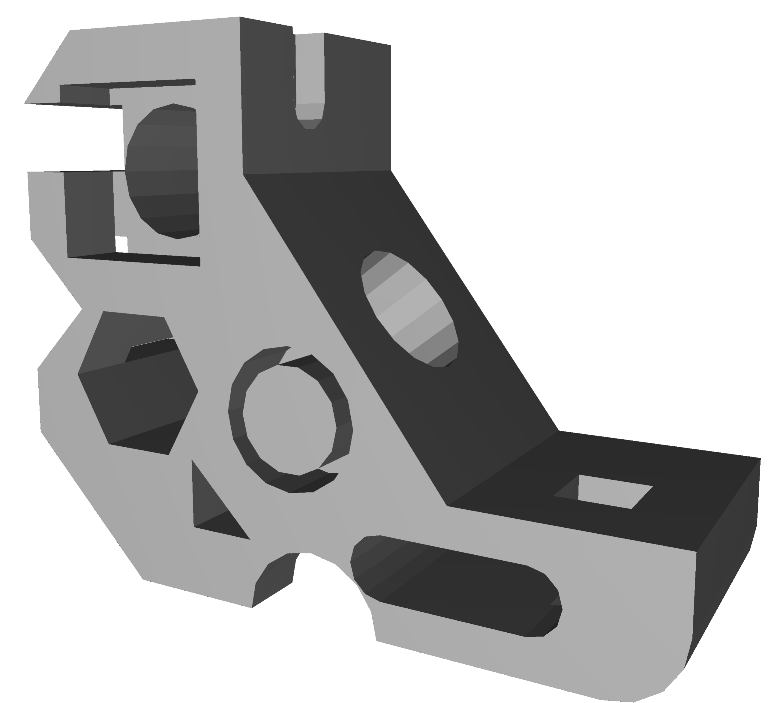
\includegraphics[width=0.6\linewidth]{pictures/STLfile.png}
  		\caption{Chosen STL-file for testing the individual pre-processing steps}
  		\label{fig:STLfile}
  	\end{center}
  \end{figure}
\subsection{Adjusting Orientation} 
Figure \ref{fig:STLfile} shows the STL-life in a unedited orientation. The Z-axis is chosen as the preferred viewing point after turning the object. The threshold for turning a area facing the axis, is set to 10\%. That means that combined facets, that lie in parallel planes and as a sum make up less than 10\%, were not viewed as potential planes that could contain features. The result of this step are shown in figure \ref{fig:TURNED1} and figure \ref{fig:TURNED2}. In total 3 STL-files are used in the subsequent steps.
\begin{figure}[H]
	\begin{center}
		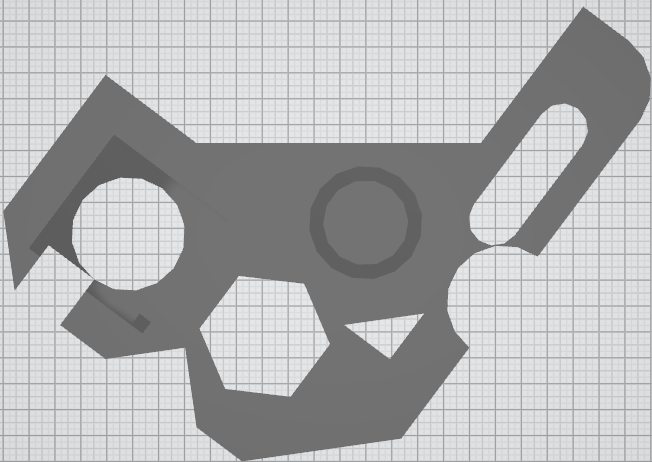
\includegraphics[width=0.6\linewidth]{pictures/TURN1.png}
		\caption{Positioning of the objects after turning the largest sloped area to the selected viewing position.}
		\label{fig:TURNED1}
	\end{center}	
\end{figure} 
\begin{figure}[H]
	\begin{center}
		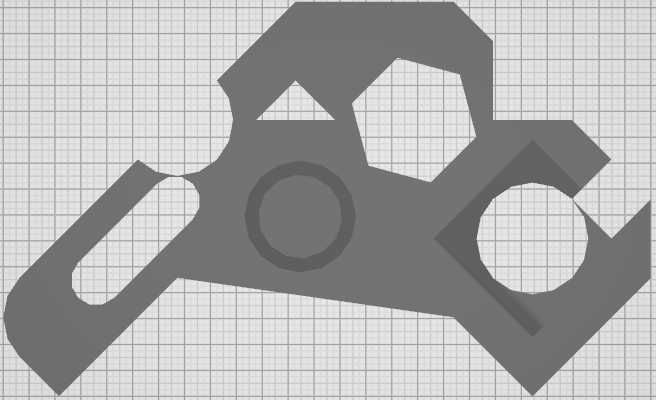
\includegraphics[width=0.6\linewidth]{pictures/TURN2.png}
		\caption{Positioning of the objects after turning the second largest sloped area to the selected viewing position.}
		\label{fig:TURNED2}
	\end{center}	
\end{figure} 
\subsection{Voxelization and Segmentation}
The minimal distance between 2 vertices in the STL-file is 0.12mm. The absolute dimensions are 100mm in X, 80mm in Y and 20mm in Z. By the proposed rule, the required resolution is set to 830 voxels, which is represented by the 830 pixels in the X axis of the output images. That means, that each picture can have a maximum dimension of 830 by 830 pixels.  The voxelizing-algorithm takes 21.2 seconds to voxelise all 3 STL-files. The results are saved as 3 separate ".npy" files that combined take up 880MB of memory. \newline

Each file is now sequentially red into memory and looped over from every direction to create the necessary main-pictures. 6 pictures are created from the original STL-file, that did not undergo rotation, and one of each from the Z-axis viewing-angle, that were turned. The result is shown in figure \ref{fig:HDRESULT}, where the last two pictures are from the tured STL-file. This process step takes 244 seconds to complete. Due to the nature of looping over all elements in a 3D-array, this can have a significant performance impact in regards to execution time.\newline

The starting-dimension for subdividing the main pictures is set to 64 pixels. The overlap is set to 66,6\% between two sub-pictures, and the increase of the dimension for every subdivision was set to 33 pixels. That means, that each picture was segmented in sub-pictures with the dimension of 64 pixel, 97 pixel, 130 pixel and so on. This result in a total of 420 images when segmenting the picture that shows the front of the STL-file, that has a resolution of 830 by 829 pixels.

After each individual picture is segmented into sub-pictures, starting from 64 pixels and ranging up to their maximum respective dimension, the over-sized pictures are scaled down into 64 by 64 pixel. One additional step is added here: all pictures that only contain the same pixel-value on all pixel are removed. They do not contain any information and therefore are not necessary to analyze.

The result of the segmentation are 9800 individual .png files that take up 20 MB. This process step takes 75 seconds to complete. Figure \ref{fig:segmented} shows how the sub-pictures are shown in the file explorer and their obvious overlap between them.
\begin{figure}[H]
	\begin{center}
		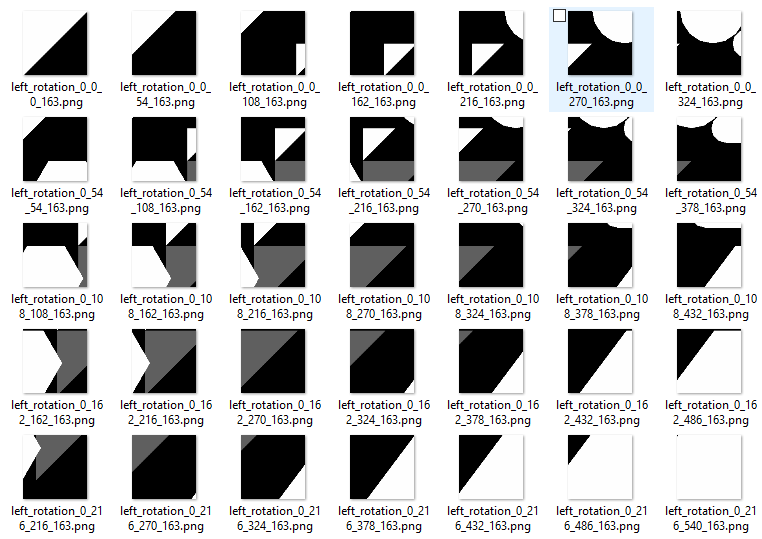
\includegraphics[width=0.9\linewidth]{pictures/segments.png}
		\caption{Sub-pictures as shown in the windows explorer}
		\label{fig:segmented}
	\end{center}
\end{figure}
  
\subsection{Recognition}
\subsection{Reconstruction}

\section{Results and Discussion}
\begin{figure}
	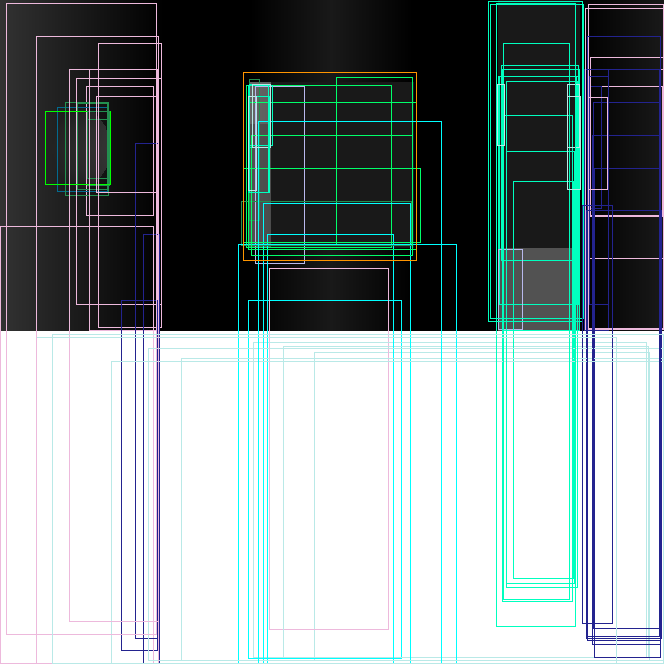
\includegraphics[width=.24\textwidth]{pictures/1.png}\hfill
	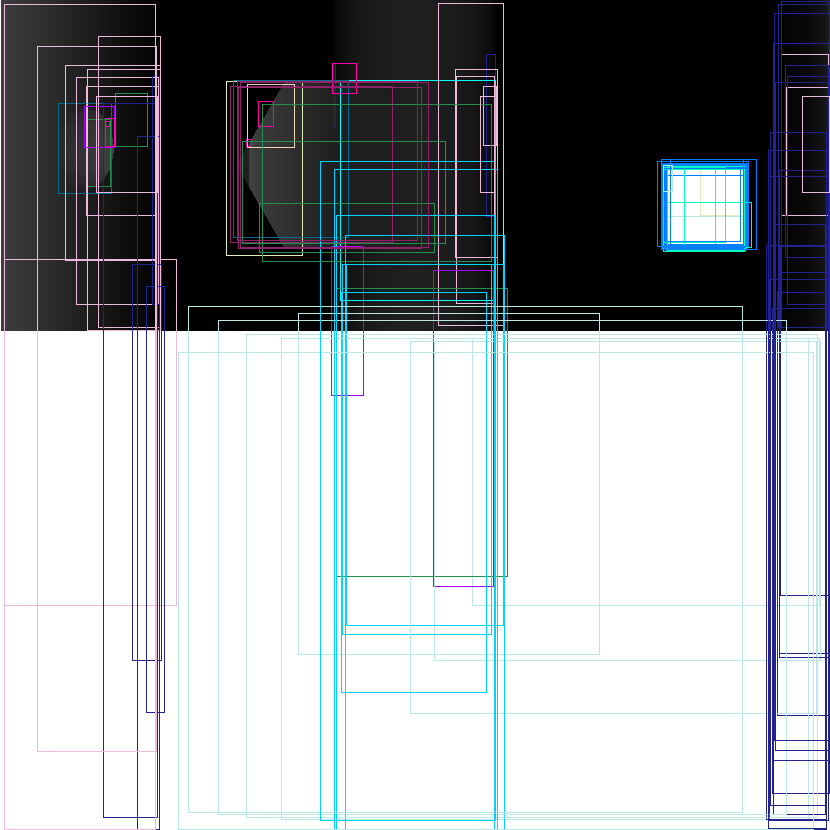
\includegraphics[width=.24\textwidth]{pictures/2.png}\hfill
	\\[\smallskipamount]
	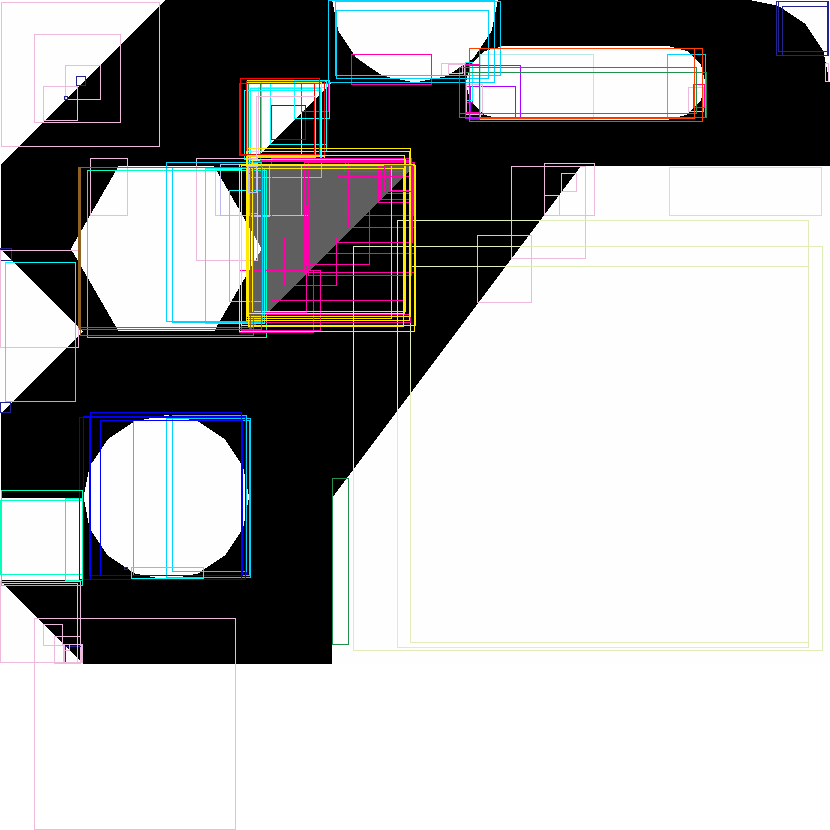
\includegraphics[width=.24\textwidth]{pictures/3.png}\hfill
	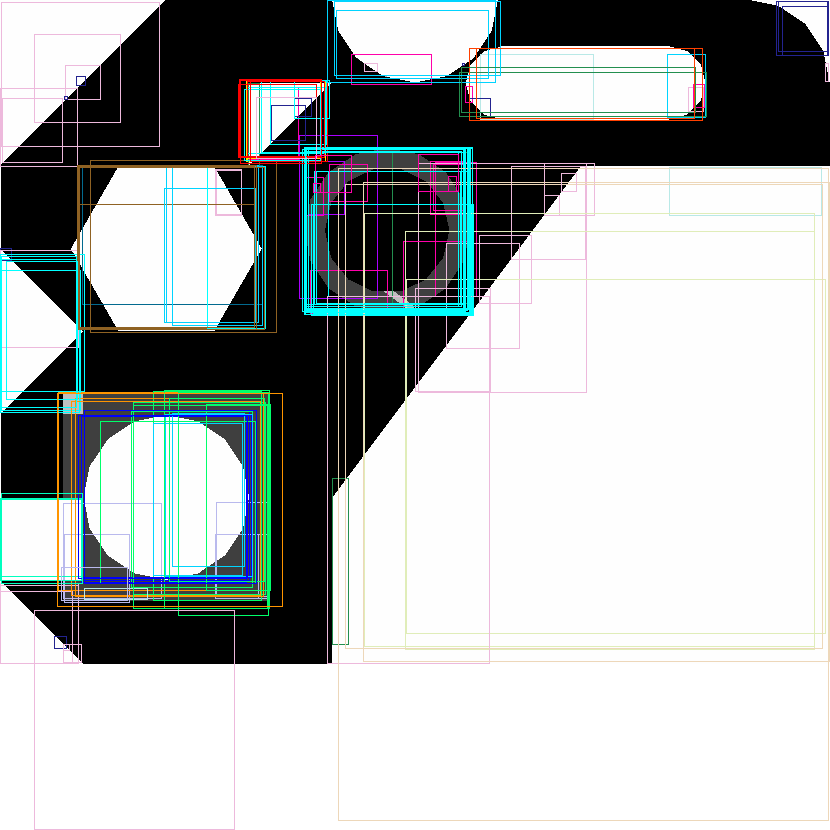
\includegraphics[width=.24\textwidth]{pictures/4.png}\hfill
	\\[\smallskipamount]
	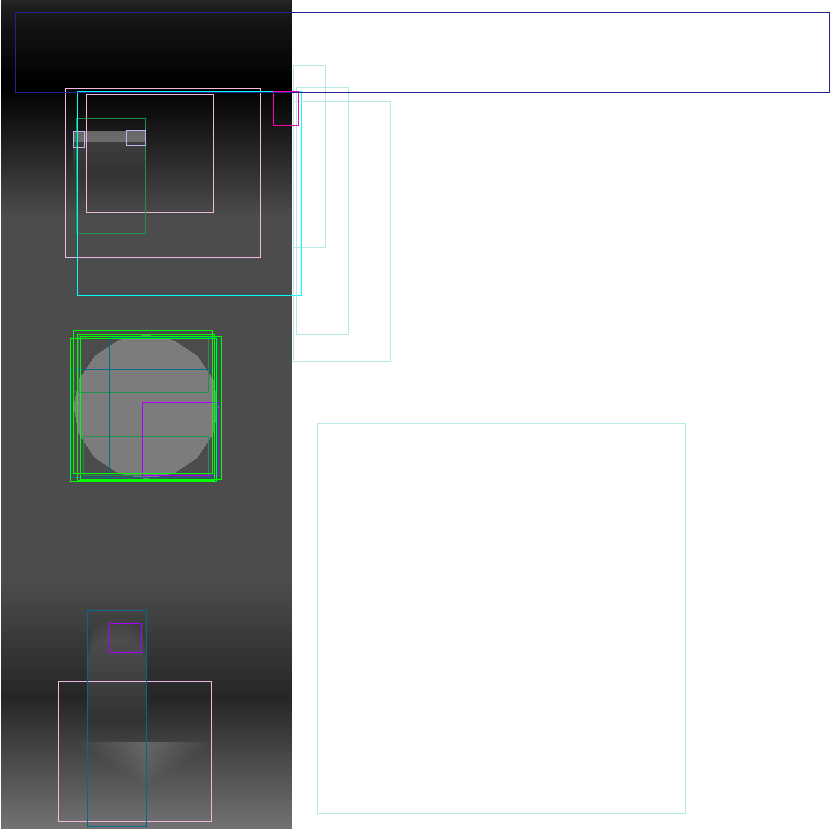
\includegraphics[width=.24\textwidth]{pictures/5.png}\hfill
	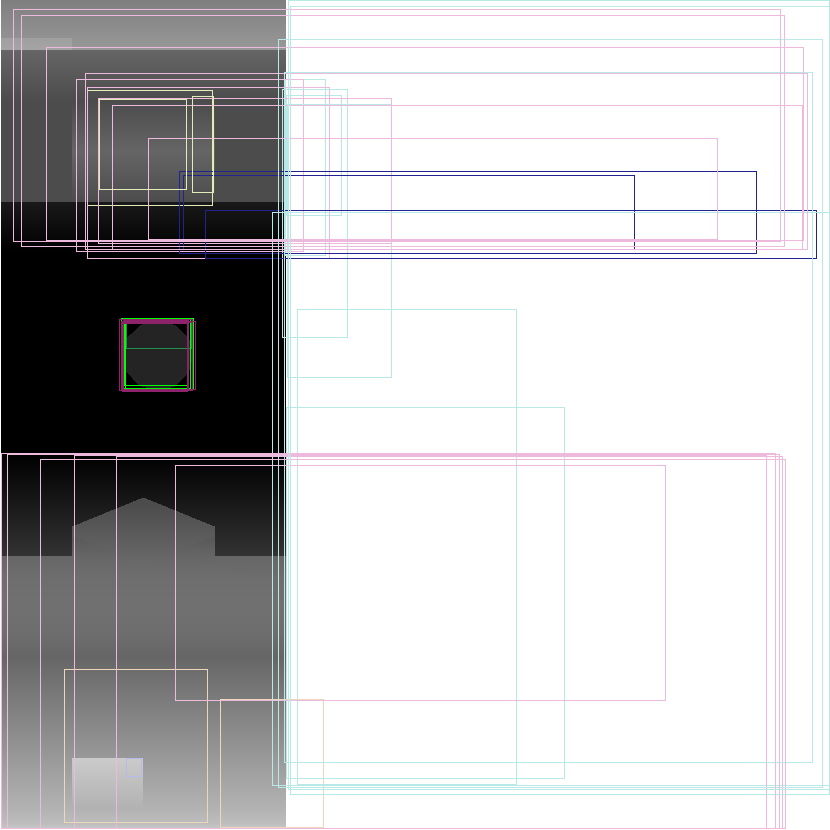
\includegraphics[width=.24\textwidth]{pictures/6.png}\hfill
	\\[\smallskipamount]
	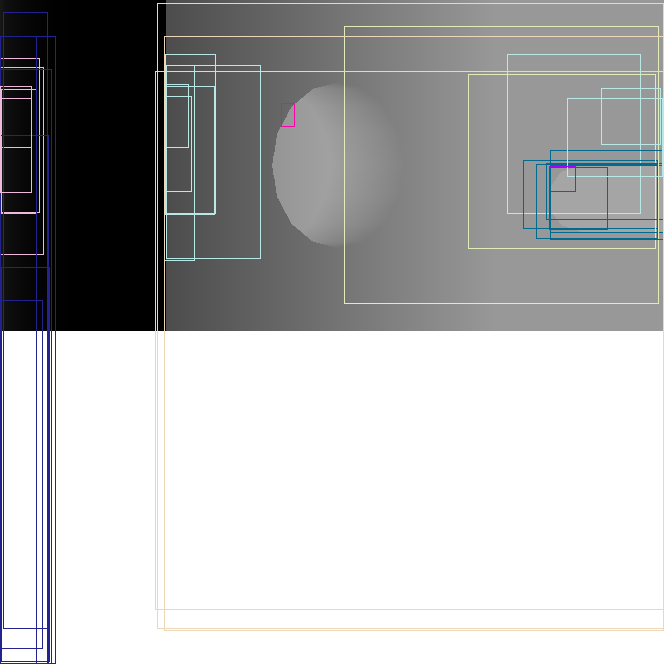
\includegraphics[width=.24\textwidth]{pictures/7.png}\hfill
	\caption{Some images}\label{fig:foobar}
\end{figure}
x
\section{Future Work}
Having the previously described process is a necessary step to improving manufacturing. But more work has to be done to solve all problems that can arise from more difficult geometries. 

To ensure the capability of working witch all possible STL-files, more features have to be added into the repertoire of the NN. As an example: bosses of various shapes, threads and stiffening ribs. 

Further, it has to be analyzed how each feature can be made ot of multiple features and how this can impact tool-path planning. As an example a T-Slot is build by combining a through slot with a through pocket. Additionally it may be beneficial to understand how features are detected on slopes. 

Finally, to increase the speed of the recognition process a faster way of recognizing the features on multiple resolution levels is required, as time efficiency is the baseline of just-in-time manufacturing. One possible option for that would be to eliminate the offloading and reloading of the used data from memory.


\section*{}
\bibliographystyle{acm}
\bibliography{REF.bib}
\section*{Appendix}


\begin{figure}
	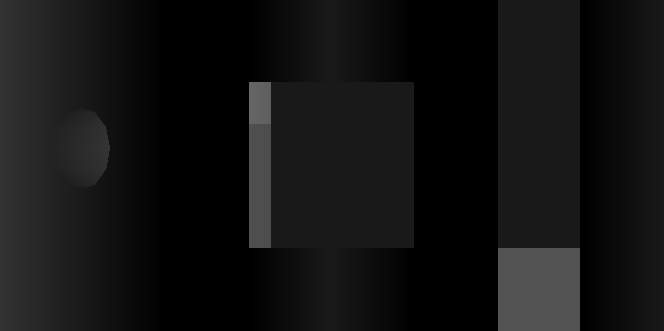
\includegraphics[width=.24\textwidth]{pictures/HD_pictures/HD_bottom_rotation_0.png}
	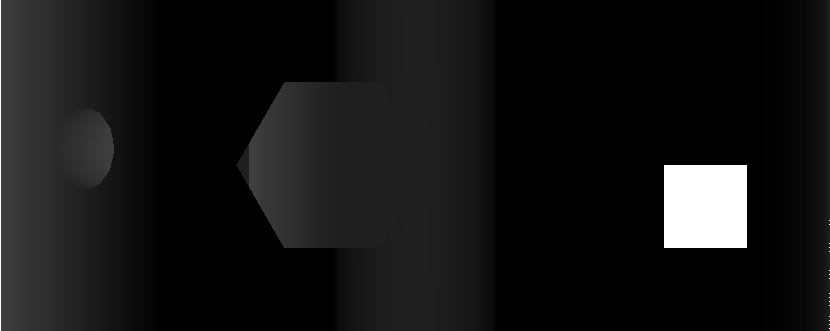
\includegraphics[width=.24\textwidth]{pictures/HD_pictures/HD_front_rotation_0.png}
	\\[\smallskipamount]
	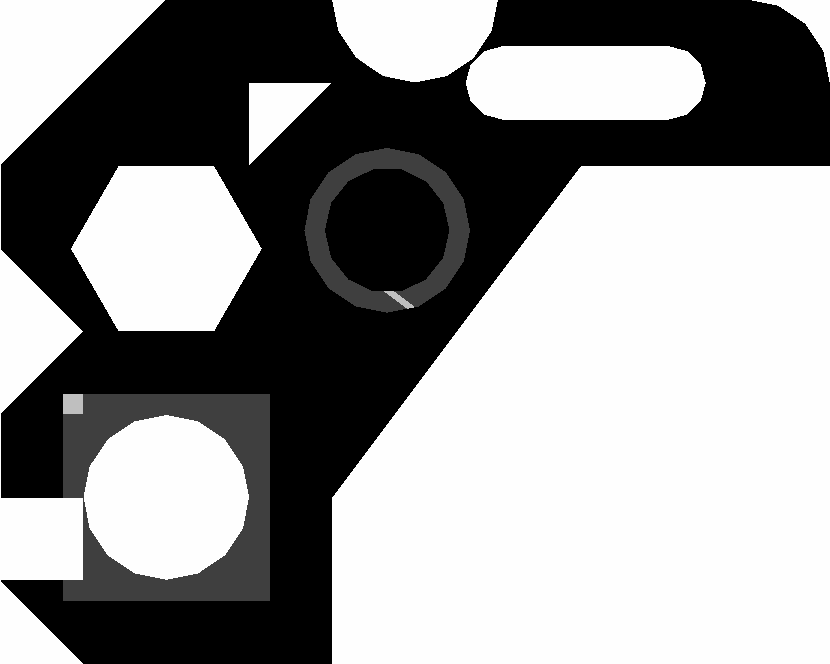
\includegraphics[width=.24\textwidth]{pictures/HD_pictures/HD_right_rotation_0.png}
	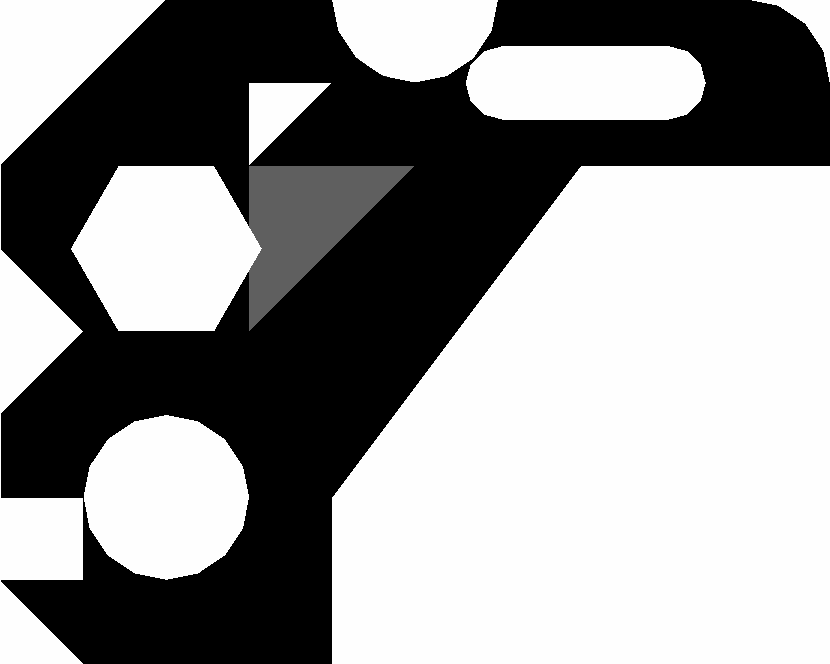
\includegraphics[width=.24\textwidth]{pictures/HD_pictures/HD_left_rotation_0.png}
	\\[\smallskipamount]
	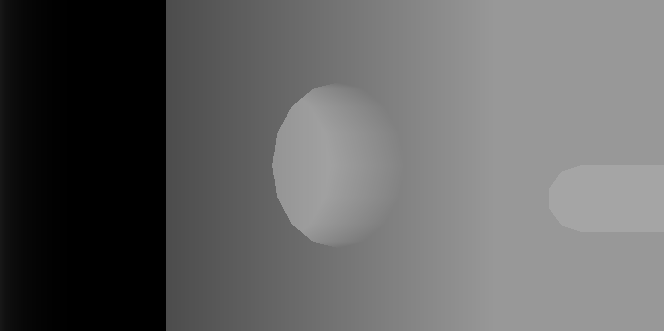
\includegraphics[width=.24\textwidth]{pictures/HD_pictures/HD_top_rotation_0.png}
	
\includegraphics[width=.24\textwidth]{pictures/HD_pictures/HD_back_rotation_0.png}
		\\[\smallskipamount]
	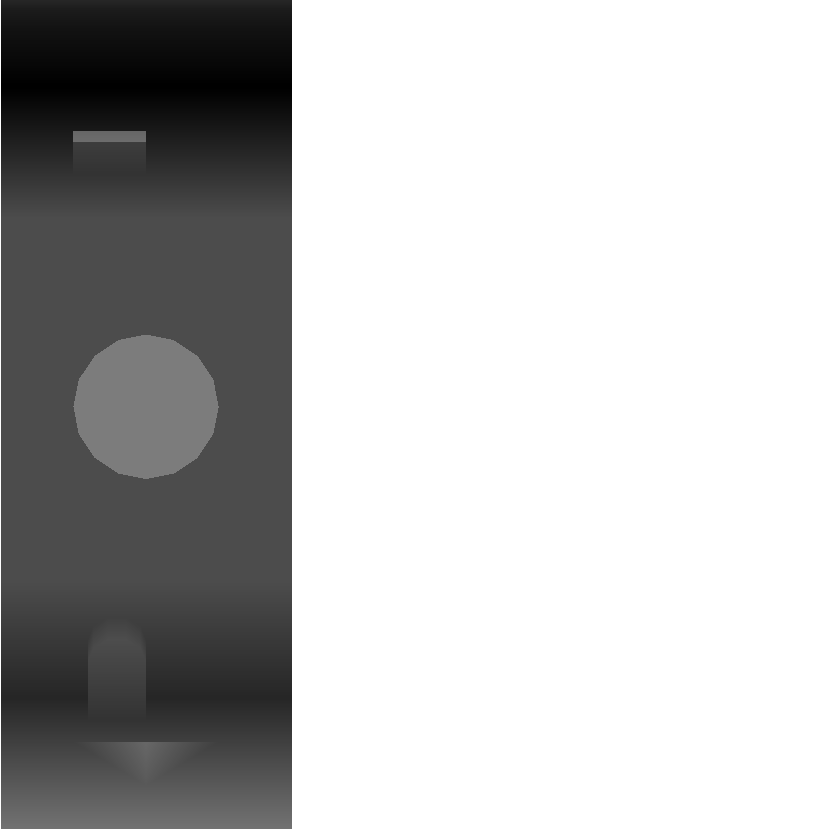
\includegraphics[width=.24\textwidth]{pictures/HD_pictures/HD_right_rotation_1.png}
	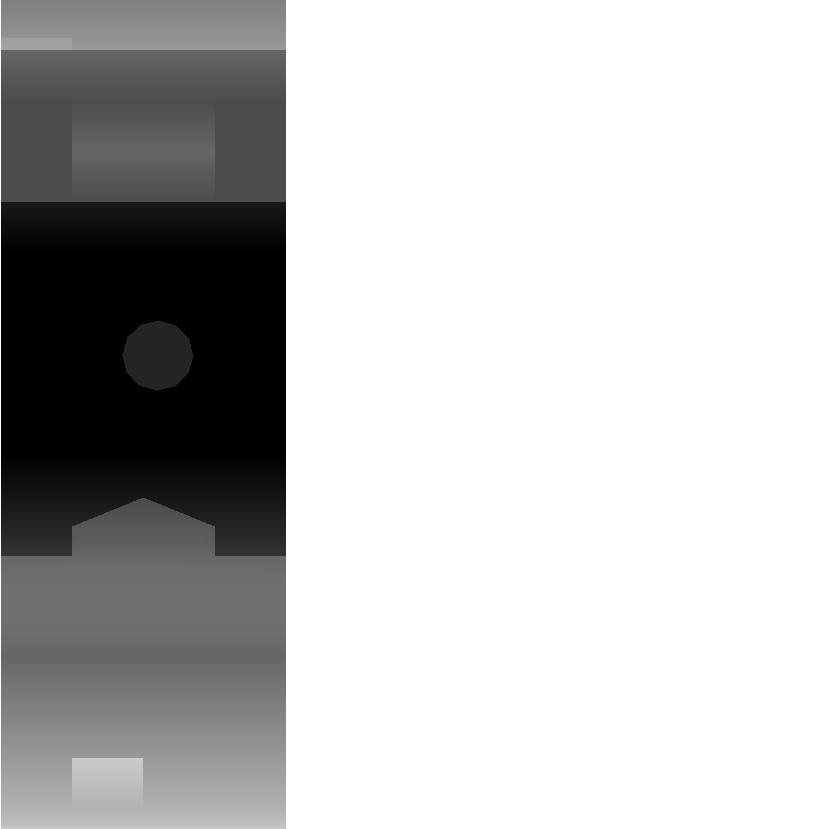
\includegraphics[width=.24\textwidth]{pictures/HD_pictures/HD_right_rotation_2.png}
	\caption{Some images}\label{fig:HDRESULT}
\end{figure}


\end{document}
